\chapter{User documentation}
\label{ch:user}

In this section I will show you how you can use the \textbf{git-qtk} (Git Query Tool Kit) which where created to solve these problems. 
The kit contains three tool and one plugin:

\begin{itemize}
\item Git History Parser. (HP)
\item Query Tool. (QT)
\item Command Line Interface. (CLI)
\item Git Plugin. (GP)
\end{itemize}

\section{System requirements}
The software is written in JavaScript and uses Node.js\cite{node.js} as runtime environment.

\subsection{Node.js and NPM}
Node.js is runtime environment that runs on the V8 engine and executes JavaScript code outside a web browser. 
NPM is the Node Package Manager which is a powerful tool to manage package dependencies. NPM has more than 1 million package\cite{npm-count} already. \newline

Users are required to download and install the \textbf{v14.x.x} version of Node.js with the packaged NPM which can be done by visiting the official website:\newline
\url{https://nodejs.org/download/release/latest-v14.x/}
\newline 

Note that this specified version is needed because of a dependency related to node-gyp\cite{node-gyp-14}
 
\subsection{Git}
For managing Git repositories a stable version Git is also required to be installed. It can be downloaded here:\newline 
\url{https://git-scm.com/}
 
\subsection{Operating system}
Node.js and Git is platform independent, it can be used on most of the modern version of Windows and Unix based operating systems.\newline

There is no official minimum system requirements for node, for running this tool it recommended to have:

\begin{itemize}
	\item x86 CPU with at least 2 vCPUs
	\item At least 8 GB of RAM
	\item At least 10 GB of storage  
	\item Internet Connection (For first time use or cloning repository over the internet)
\end{itemize}


\section{Installation}
The software comes as a Node.js package, which can be installed in multiple different way. 
The installation is done by the Node Package Manager 

Notice: Administrator privileges may be needed in Windows OS.

\subsection{From source files}
If you want to install the toolkit from a local copy of the project you will have to extract the source to a folder. 
Then you have to install the dependencies with npm.
To do that run this command:

\textbf{npm install . --global}

\subsection{From the GitHub repository}
The repository is version controlled with Git, and the project is available publicly on GitHub. 
To install the toolkit you have to run this command:

\textbf{npm install https://github.com/imdonix/git-qtk.git --global}

\section{Basics TODo} (2)

\section{The query language} (0.5)

The toolkit provides an easy way to search in the history.
The query is based on YAML\cite{yaml} markup language which is a is a human-friendly data serialization language for all programming languages. 
By defineing the following tags you can manipulate the query as you wish.


\subsection{From} (0.5)

In the \textit{From} tag you have to define which models you want to include in your search.
This tag is required.
You can define it with the following rules:

\begin{itemize}
	\item A model can be selected by adding the model name to the tag.
	\item Multiple model can be added by separating them with the \textbf{;} delimiter.
	\item A single model can be added multiple time by renaming it which can be done by adding a "nickname" after the model name.
\end{itemize}

Note: Based on the givven models the tool will create a subset of the needed plguins for performance reason.

\subsection{Select} (0.5)

The \textit{Select} tag is used to create a subset of the result and process it from the search:
This tag is required.
You can define it with the following rules:

\begin{itemize}
	\item A single statement can be added with the \textbf{'{model}.{field}'} syntax.
	\item Multiple statement can be selected by separating them with the \textbf{';'} delimiter.
	\item Each statement will be interpreted and evaluated as JavaScript.
	\item The \textbf{\$} symbol is a wildcard to select all fields. 
\end{itemize}

\subsection{Where} (0.5)

The \textit{Where} tag can be used to filter records from the records.
This is an optional tag, otherwise all record will be passed.
You can define it with the following rules:

\begin{itemize}
	\item A single JavaScript statement should be provided.
	\item The record fields can be referenced as \textbf{'{model}.{field}'}
\end{itemize}

\subsubsection{Join}

// THIS SHOUD BE A DEV DOC OR NOT?

A special case of the filtering is considered as join. 
This happens if a subset of the statement looks like:\newline

\textbf{{model}.{field} == {model}.{field}}\newline

In this case the following rules applies:

\begin{itemize}
	\item If only one of the field is a key for the model then its a \textbf{Right or Left Join}
	\item If both of them are key then its a \textbf{Inner Join}
	\item If none of then is a key this will be evaluated normaly
\end{itemize}

This sub statements will be removed from the where tag and added handled separatly for performance resons

\subsection{Limit} (0.5)

The \textit{Limit} tag define how many records should be displayed to the output.
This field is optional.

\subsection{Order} (0.5)

The \textit{Order} tag will define how the records should be ordered.
This field is optional.

The following rules applies:

\begin{itemize}
	\item Descending order: \textbf{DESC}
	\item Ascending order: \textbf{ASC}
	\item A single JavaScript statement should be provided with the order key separeted by a space
	\item The record fields can be referenced as \textbf{'{model}.{field}'}
\end{itemize}

\subsection{Group} (0.5)

The \textit{Group} tag groups records that have the same values into summary records.

The following rules applies:
\begin{itemize}
	\item A single field should be added as \textbf{'{model}.{field}'}
\end{itemize}


\section{How to use the Toolkit}
The toolkit intended to be used as a library for software which provide information about the progress of a project, the performance of the co-workers and much more. But in the development phase a CLI tool is also available so implementing the specified queries can be down easily.

\subsection{As a CLI tool}
After installing the tool globally it can be tested by running the next command, this will provide all the functionally available with the CLI Tool:

\textbf{git-qtk}
\subsubsection{Version}
The version of the tool can be queried with the \textbf{-v} or \textbf{-version} flag.

\begin{figure}[H]
	\centering
	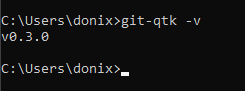
\includegraphics[width=150px]{version}
	\caption{Querying the version of the toolkit}
	\label{fig:fig-version}
\end{figure}

This will also check that a new version of the toolkit is available in the GitHub repository\cite{repo}. 

\newpage
\subsubsection{Help}
All the available command will be displayed with description when running the program with the \textbf{-h} or \textbf{-help} flag.

\begin{figure}[H]
	\centering
	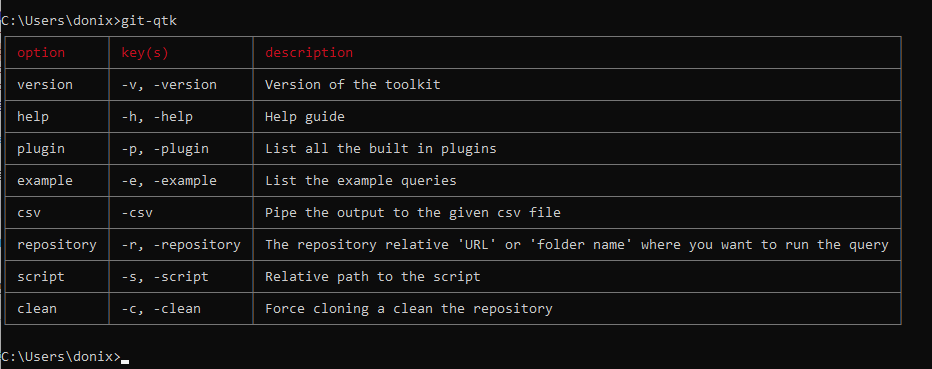
\includegraphics[width=350px]{help}
	\caption{Help of the tool}
	\label{fig:fig-help}
\end{figure}

\subsubsection{Plugin}
With the \textbf{-p} or \textbf{-plugin} flag you will be able to access all the models provided by the tool kit.

\begin{figure}[H]
	\centering
	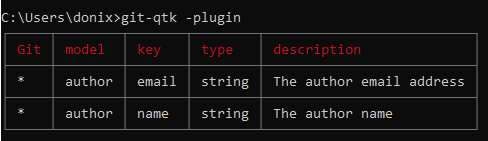
\includegraphics[width=300px]{plugin}
	\caption{List of the models provided by built in plugins}
	\label{fig:fig-plugin}
\end{figure}

\subsubsection{Examples}
To get example queries as reference you can use the \textbf{-e} or \textbf{-example} flag.

\begin{figure}[H]
	\centering
	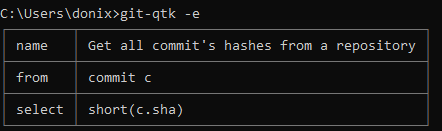
\includegraphics[width=300px]{examplee}
	\caption{An example query}
	\label{fig:fig-example}
\end{figure}

\subsubsection{Running a query}
To run a query on a specified repository must provide the following information for the tool kit:

\begin{itemize}
	\item \textbf{-r} or -\textbf{repository} to specify which repository history should be parsed. You can give a local folder relative path or a full URL which will be cloned.
	\item \textbf{-s} or -\textbf{script} to specify which query you want to run. You can give a relative path to the query file.
\end{itemize}

This will run the query on the given repository an the result will be printed to the standard output by default.

\begin{figure}[H]
	\centering
	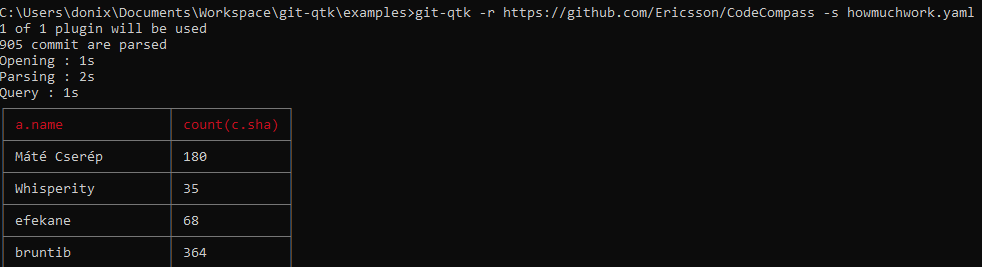
\includegraphics[width=420px]{query}
	\caption{Part of the output}
	\label{fig:fig-query}
\end{figure}


\subsection{As a Node.js library}

TODO

\subsection{Extending with plugins} (2)

TODO

\section{Use cases / Examples} (0.5)

TODO

\subsection{Use case A} (0.5)

TODO

\subsection{Use case B} (0.5)

TODO

\subsection{Use case C} (0.5)

TODO

\section{Enumerations and lists}

TODO

Etiam vel odio ante. Etiam pulvinar nibh quis massa auctor congue. Pellentesque quis odio vitae sapien molestie vestibulum sit amet et quam. Pellentesque vel dui eget enim hendrerit finibus at sit amet libero. Quisque sollicitudin ultrices enim, nec porta magna imperdiet vitae. Cras condimentum nunc dui, eget molestie nunc accumsan vel.

\begin{lstlisting}
	# Let me re-iterate ...
	const a = require('a')
	
	for i in 1 .. 10 { do-something(i) }
\end{lstlisting}


\begin{itemize}
	\item Fusce in aliquet neque, in pretium sem.
	\item Donec tincidunt tellus id lectus pretium fringilla.
	\item Nunc faucibus, erat pretium tempus tempor, tortor mi fringilla neque, ac congue ex dui vitae mauris.
\end{itemize}

Donec dapibus sodales ante, at scelerisque nunc laoreet sit amet. Mauris porttitor tincidunt neque, vel ullamcorper neque pulvinar et. Integer eu lorem euismod, faucibus lectus sed, accumsan felis. Nunc ornare mi at augue vulputate, eu venenatis magna mollis. Nunc sed posuere dui, et varius nulla. Sed mollis nibh augue, eget scelerisque eros ornare nec.

\begin{enumerate}
	\item\label{step:first} Donec pretium et quam a cursus. Ut sollicitudin tempus urna et mollis.
	\item Aliquam et aliquam turpis, sed fermentum mauris. Nulla eget ex diam.
	\item Donec eget tellus pharetra, semper neque eget, rutrum diam Step~\ref{step:first}.
\end{enumerate}

Praesent porta, metus eget eleifend consequat, eros ligula eleifend ex, a pellentesque mi est vitae urna. Vivamus turpis nunc, iaculis non leo eget, mattis vulputate tellus. Maecenas rutrum eros sem, pharetra interdum nulla porttitor sit amet. In vitae viverra ante. Maecenas sit amet placerat orci, sed tincidunt velit. Vivamus mattis, enim vel suscipit elementum, quam odio venenatis elit\footnote{Phasellus faucibus varius purus, nec tristique enim porta vitae.}, et mollis nulla nunc a risus. Praesent purus magna, tristique sed lacus sit amet, convallis malesuada magna. 

\begin{description}
	\item[Vestibulum venenatis] malesuada enim, ac auctor erat vestibulum et. Phasellus id purus a leo suscipit accumsan.
	\item[Orci varius natoque] penatibus et magnis dis parturient montes, nascetur ridiculus mus. Nullam interdum rhoncus nisl, vel pharetra arcu euismod sagittis. Vestibulum ac turpis auctor, viverra turpis at, tempus tellus.
	\item[Morbi dignissim] erat ut rutrum aliquet. Nulla eu rutrum urna. Integer non urna at mauris scelerisque rutrum sed non turpis.
\end{description}

\subsection{Lists with narrow spacing inbetween items}

Phasellus ultricies, sapien sit amet ultricies placerat, velit purus viverra ligula, id consequat ipsum odio imperdiet enim:
\begin{compactenum}
	\item Maecenas eget lobortis leo.
	\item Donec eget libero enim.
	\item In eu eros a eros lacinia maximus ullamcorper eget augue.
\end{compactenum}

\bigskip

In quis turpis metus. Proin maximus nibh et massa eleifend, a feugiat augue porta. Sed eget est purus. Duis in placerat leo. Donec pharetra eros nec enim convallis:
\begin{compactitem}
	\item Pellentesque odio lacus.
	\item Maximus ut nisl auctor.
	\item Sagittis vulputate lorem.
\end{compactitem}

\bigskip

Vestibulum ante ipsum primis in faucibus orci luctus et ultrices posuere cubilia Curae; Sed lorem libero, dignissim vitae gravida a, ornare vitae est.
\begin{compactdesc}
	\item[Cras maximus] massa commodo pellentesque viverra.
	\item[Morbi sit] amet ante risus. Aliquam nec sollicitudin mauris
	\item[Ut aliquam rhoncus sapien] luctus viverra arcu iaculis posuere
\end{compactdesc}


\section{Images and figures}

Aliquam vehicula luctus mi a pretium. Nulla quam neque, maximus nec velit in, aliquam mollis tortor. Aliquam erat volutpat. Curabitur vitae laoreet turpis. Integer id diam ligula. Nulla sodales purus id mi consequat, eu venenatis odio pharetra. Cras a arcu quam. Suspendisse augue risus, pulvinar a turpis et, commodo aliquet turpis. Nulla aliquam scelerisque mi eget pharetra. Mauris sed posuere elit, ac lobortis metus. Proin lacinia sit amet diam sed auctor. Nam viverra orci id sapien sollicitudin, a aliquam lacus suscipit, Figure~\ref{fig:example-1}:

\begin{figure}[H]
	\centering
	
\includegraphics[width=0.6\textwidth,height=100px]{elte_cimer_szines}
	\caption{Quisque ac tincidunt leo}
	\label{fig:example-1}
\end{figure}

\subsection{Framing figures}

Ut aliquet nec neque eget fermentum. Cras volutpat tellus sed placerat elementum. Quisque neque dui, consectetur nec finibus eget, blandit id purus. Nam eget ipsum non nunc placerat interdum.

\begin{figure}[H]
	\centering
	
\includegraphics[width=0.6\textwidth,height=100px,frame]{elte_cimer_szines}
	\caption{Quisque ac tincidunt leo}
\end{figure}

\subsection{Subfigures}

In non ipsum fermentum urna feugiat rutrum a at odio. Pellentesque habitant morbi tristique senectus et netus et malesuada fames ac turpis egestas. Nulla tincidunt mattis nisl id suscipit. Sed bibendum ac felis sed volutpat. Nam pharetra nisi nec facilisis faucibus. Aenean tristique nec libero non commodo. Nulla egestas laoreet tempus. Nunc eu aliquet nulla, quis vehicula dui. Proin ac risus sodales, gravida nisi vitae, efficitur neque, Figure~\ref{fig:example-2}:

\begin{figure}[H]
	\centering
	\subcaptionbox{Vestibulum quis mattis urna}{
		
\includegraphics[width=0.45\linewidth]{elte_cimer_szines}}
	\hspace{5pt}
	\subcaptionbox{Donec hendrerit quis dui sit amet venenatis}{
		
\includegraphics[width=0.45\linewidth]{elte_cimer_szines}}
	\caption{Aenean porttitor mi volutpat massa gravida}
	\label{fig:example-2}
\end{figure}

Nam et nunc eget elit tincidunt sollicitudin. Quisque ligula ipsum, tempor vitae tortor ut, commodo rhoncus diam. Pellentesque habitant morbi tristique senectus et netus et malesuada fames ac turpis egestas. Phasellus vehicula quam dui, eu convallis metus porta ac.


\section{Tables}

Nam magna ex, euismod nec interdum sed, sagittis nec leo. Nam blandit massa bibendum mattis tristique. Phasellus tortor ligula, sodales a consectetur vitae, placerat vitae dolor. Aenean consequat in quam ac mollis. 

\begin{table}[H]
	\centering
	\begin{tabular}{ | m{0.25\textwidth} | m{0.65\textwidth} | }
		\hline
		\textbf{Phasellus tortor} & \textbf{Aenean consequat} \\
		\hline \hline
		\emph{Sed malesuada} & Aliquam aliquam velit in convallis ultrices. \\
		\hline
		\emph{Purus sagittis} &  Quisque lobortis eros vitae urna lacinia euismod. \\
		\hline
		\emph{Pellentesque} & Curabitur ac lacus pellentesque, eleifend sem ut, placerat enim. Ut auctor tempor odio ut dapibus. \\
		\hline
	\end{tabular}
	\caption{Maecenas tincidunt non justo quis accumsan}
	\label{tab:example-1}
\end{table}

\subsection{Multi rows and multi columns}

Mauris a dapibus lectus. Vestibulum commodo nibh ante, ut maximus magna eleifend vel. Integer vehicula elit non lacus lacinia, vitae porttitor dolor ultrices. Vivamus gravida faucibus efficitur. Ut non erat quis arcu vehicula lacinia. Nulla felis mauris, laoreet sed malesuada in, euismod et lacus. Aenean at finibus ipsum. Pellentesque dignissim elit sit amet lacus congue vulputate.

\begin{table}[htb]
	\centering
	\begin{tabular}{ | c | r | r | r | r | r | r | }
		\hline
		\multirow{2}{*}{\textbf{Quisque}} & \multicolumn{2}{ c | }{\textbf{Suspendisse}} & \multicolumn{2}{ c | }{\textbf{Aliquam}} & \multicolumn{2}{ c | }{\textbf{Vivamus}} \\
		\cline{2-7}
		& Proin & Nunc & Proin & Nunc & Proin & Nunc \\
		\hline \hline		
		Leo & 2,80 MB & 100\% & 232 KB & 8,09\% & 248 KB & 8,64\% \\
		\hline
		Vel & 9,60 MB & 100\% & 564 KB & 5,74\% & 292 KB & 2,97\% \\
		\hline
		Auge & 78,2 MB & 100\% & 52,3 MB & 66,88\% & 3,22 MB & 4,12\% \\
		\hline 
	\end{tabular}
	\caption[Rövid cím a táblázatjegyzékbe]{Vivamus ac arcu fringilla, fermentum neque sed, interdum erat. Mauris bibendum mauris vitae enim mollis, et eleifend turpis aliquet.}
	\label{tab:example-2}
\end{table}

\subsection{Long tables over multiple pages}

Nunc porta placerat leo, sit amet porttitor dui porta molestie. Aliquam at fermentum mi. Maecenas vitae lorem at leo tincidunt volutpat at nec tortor. Vivamus semper lacus eu diam laoreet congue. Vivamus in ipsum risus. Nulla ullamcorper finibus mauris non aliquet. Vivamus elementum rhoncus ex ut porttitor.

\begin{center}
	\begin{longtable}{ | p{0.3\textwidth} | p{0.7\textwidth} | }
		
		\hline
		\multicolumn{2}{|c|}{\textbf{Praesent aliquam mauris enim}}
		\\ \hline
		
		\emph{Suspendisse potenti} & \emph{Lorem ipsum dolor sit amet}
		\\ \hline \hline
		\endfirsthead % table header on first page
		
		\hline
		\emph{Suspendisse potenti} & \emph{Lorem ipsum dolor sit amet}
		\\ \hline \hline
		\endhead % table header on further pages
		
		\hline
		\endfoot % table footer on previous pages
		
		\endlastfoot % table footer on last page
		
		\emph{Praesent}
		& Nulla ultrices et libero sit amet fringilla. Nunc scelerisque ante tempus sapien placerat convallis.
		\\ \hline
		
		\emph{Luctus}
		& Integer hendrerit erat massa, non hendrerit risus convallis at. Curabitur ultrices, justo in imperdiet condimentum, neque tortor luctus enim, luctus posuere massa erat vitae nibh.
		\\ \hline
		
		\emph{Egestas}
		& Duis fermentum feugiat augue in blandit. Mauris a tempor felis. Pellentesque ultricies tristique dignissim. Pellentesque aliquam semper tristique. Nam nec egestas dolor. Vestibulum id elit quis enim fringilla tempor eu a mauris. Aliquam vitae lacus tellus. Phasellus mauris lectus, aliquam id leo eget, auctor dapibus magna. Fusce lacinia felis ac elit luctus luctus.
		\\ \hline
		
		\emph{Dignissim}
		& Praesent aliquam mauris enim, vestibulum posuere massa facilisis in. Suspendisse potenti. Nam quam purus, rutrum eu augue ut, varius vehicula tellus. Fusce dui diam, aliquet sit amet eros at, sollicitudin facilisis quam. Phasellus tempor metus vel augue gravida pretium. Proin aliquam aliquam blandit. Nulla id tempus mi. Fusce in aliquam tortor.
		\\ \hline
		
		\emph{Pellentesque}
		& Donec felis nibh, imperdiet a arcu non, vehicula gravida nibh. Quisque interdum sapien eu massa commodo, ac elementum felis faucibus.
		\\ \hline
		
		\emph{Molestie}
		& Cras ullamcorper tellus et auctor ultricies. Maecenas tincidunt euismod lectus nec venenatis. Suspendisse potenti. Pellentesque pretium nunc ut euismod cursus. Nam venenatis condimentum quam. Curabitur suscipit efficitur aliquet. Interdum et malesuada fames ac ante ipsum primis in faucibus.
		\\ \hline
		
		\emph{Vivamus semper}
		& In purus purus, faucibus eu libero vulputate, tristique sodales nunc. Nulla ut gravida dolor. Fusce vel pellentesque mi, vel efficitur eros. Nunc vitae elit tellus. Sed vestibulum auctor consequat. 
		\\ \hline
		
		\emph{Condimentum}
		& Nulla scelerisque, leo et facilisis pretium, risus enim cursus turpis, eu suscipit ipsum ipsum in mauris. Praesent eget pulvinar ipsum, suscipit interdum nunc. Nam varius massa ut justo ullamcorper sollicitudin. Vivamus facilisis suscipit neque, eu fermentum risus. Ut at mi mauris.
		\\ \hline
		
		\caption{Praesent ullamcorper consequat tellus ut eleifend}
		\label{tab:example-3}		
	\end{longtable}
\end{center}